\documentclass[a4,12pt]{article}

\usepackage[utf8]{inputenc}
\usepackage[spanish]{babel}
\usepackage[margin=1.5cm]{geometry}
\usepackage{graphicx}
\usepackage{color}
\usepackage{import}
\usepackage{float }



\usepackage{hyperref}

\parindent 0em

%\usepackage{times}
\renewcommand{\familydefault}{\sfdefault}

\title{Resolución de problemas a GNU OCTAVE}
\author{Lamya Hafs}
%\date{}

\begin{document}

\maketitle
\bigskip
\bigskip
\bigskip
\begin{figure}[H]
  \centering
    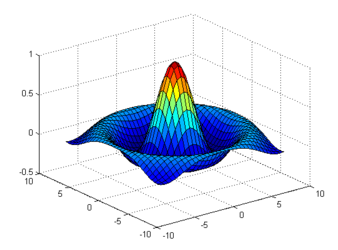
\includegraphics{imagenes/octave}
\end{figure}
\newpage

\maketitle

\begin{abstract}
El documento explica como se ha conseguido resolver problemas mediante el software GNU Octave, se ha elegido dos problemas.\\
- Problema de programacion lineal propuesto en la parte de MatApl "El problema de dieta".\\
- Problema de ordenamiento rápido "Quicksort".\\

\end{abstract}

\tableofcontents
\newpage

\section{El problema de dieta}

\subsection{Discripción del problema}
Se desea añadir a la dieta de ciertos animales de granja cantidades extra de tiamina, fósforo y hierro.\\
Para ello en el mercado existen dos preparados en polvo diferentes: Fosfatón y Ferroforo. Estos
contienen los nutrientes en las cantidades que se indican a continuación. Cada onza de Ferroforo
contiene 0.15 mg de tiamina, 0.75 mg de fósforo y 1.30 mg de hierro. Cada onza de Fosfatón contiene 0.10 mg de tiamina, 1.70 mg de fósforo y 1.10 mg de hierro. Deseamos que cada animal reciba al día, al menos 1.00 mg de tiamina, 7.50 mg de fósforo y 10.00 mg de hierro.\\
El costo de cada onza de Ferroforo es de 0.02 euros y el de Fosfatón es de 5/3 de céntimo de euro poronza. Determinar las cantidades de Ferroforo y Fosfatón que debemos suministrar a cada animal de forma que el costo de este suplemento a la dieta sea mínimo.\\

\subsection{Solución}
En primer lugar expresamos los datos del problema en forma de tabla, lo que nos dará una mejor
perspectiva de los mismos:\\

\begin{center}
\begin{tabular}{|c|c|c|c|c|} \hline
\textbf{Ingredientes}   &  \textbf{Tiamina}  &  \textbf{Fósforo} &  \textbf{Hierro}  &  \textbf{Coste de los igredientes} \\ \hline
Ferroforo  & 0.15 mg/oz  &  0.75 mg/oz & 1.30 mg/oz  &  2 ct/oz  \\  \hline
Fosfatón  & 0.10 mg/oz  &  1.70 mg/oz & 1.10 mg/oz  &  573 ct/oz  \\  \hline
\end{tabular}
\end{center}

• Definición de las variables del problema:\\
Sean x1 y x2 las cantidades, en onzas, de Ferroforo y Fosfatón, respectivamente, que debemos añadir a la dieta de los animales diariamente.\\
• Restricciones del problema:\\
Al echar a la dieta x1 onzas de Ferroforo y x2 onzas de Fosfatón estaríamos proporcionando a la misma el siguiente aporte nutricional diario:\\

\begin{verbatim}
                  0.15 x1 + 0.10 x2 mg de Tiamina
                  0.75 x1 + 1.70 x2 mg de Fósforo
                  1.30 x1 + 1.10 x2 mg de Hierro
\end{verbatim}
                  
Como deseamos que cada animal reciba al día, al menos 1.00 mg de tiamina, 7.50 mg de fósforo y 10.00 mg de hierro. Deberemos imponer las siguientes restricciones:\\

\begin{verbatim}
                  0.15 x1 + 0.10 x2 >= 1.00
                  0.75 x1 + 1.70 x2 >= 7.50
                  1.30 x1 + 1.10 x2 >= 10.00
\end{verbatim}
                  
• Restricciones de no negatividad:\\
Tal y como hemos definido las variables del problema no tiene ningún sentido que éstas tomen valores negativos. De manera que también impondremos las restricciones:\\

\begin{verbatim}
         x1 >= 0
         x2 >= 0
\end{verbatim}

Estas restricciones se suelen expresar de forma conjunta del siguiente modo:\\
\begin{verbatim}
         x1 , x2 >= 0
\end{verbatim}

y se les llama las restricciones de no negatividad.\\

• Definición de la función que representa el objetivo que pretendemos alcanzar:\\
Es lógico pensar que habrá muchas pares de valores (x1, x2) que cumplirán todas las restricciones del problema. Cada uno de estos pares de valores (x1,x2), que significa echar, diariamente, a la dieta de los animales x1 onzas de Ferroforo y x2 onzas de Fosfatón, , tendrá un costo de 2 x1 + 5/3 x2 céntimos de euro.\\

Luego si llamamos z = 2 x1 + 5/3 x2 , z representa el costo, en céntimos de euro, asociado al par (x1, x2) de valores de las variables.\\

Es evidente que nuestro objetivo será determinar el par (x1, x2) que cumpliendo todas las restricciones del problema haga mínimo el valor de la función z.\\

Luego el problema que hemos de resolver lo podemos expresar del siguiente modo:\\
         
\begin{figure}[H]
  \centering
    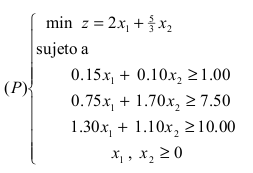
\includegraphics{imagenes/SolucionDieta}
\end{figure}

\subsection{Solución en OCTAVE}
 
\textbf {La introduccion de los dados del problema en OCTAVE} apartir del resultado conseguido  tenemos que resolver tanto x1 como x2 para encontrar el coste minimo.\\
Para ello seguimos los pasos siguientes : \\

• Primero se introduce en Octave los factores de la primera parte de cada ecuación .\\
\begin{verbatim}
octave-3.2.4:1> a =[0.15,0.10;0.75,1.70;1.30,1.10]
a =

   0.15000   0.10000
   0.75000   1.70000
   1.30000   1.10000
   
\end{verbatim}

• Segungo se introduce los factores de la segunda parte de cada ecuación.\\
\begin{verbatim}
octave-3.2.4:2> b=[1;7.5;10]
b =

    1.0000
    7.5000
   10.0000
   
\end{verbatim}

• los valores resueltos con Octave de x1 y x2 son :\\
\begin{verbatim}
octave-3.2.4:3> a\b
ans =

   6.2983
   1.6347
\end{verbatim}

\end{document}

